\documentclass[lualatex,handout]{beamer}
\setbeamertemplate{footline}[frame number]
\usepackage{luatexja}
\usepackage{amsmath,amssymb}

%\usetheme{Berlin}
\usecolortheme{rose}

\usepackage{tikz}
\usepackage{pgfplots}
\pgfplotsset{compat=1.18}

%\usepackage[haranoaji]{luatexja-preset}
\usepackage[deluxe,ipaex]{luatexja-preset}
\renewcommand{\kanjifamilydefault}{\gtdefault}
%\setmainjfont{HaranoAjiGothic-Regular}

\usepackage{unicode-math}
%\setmathfont{Fira Math}
\setmathfont{STIX Two Math}
\setmathfont{STIX Two Math}[range=bfup/{Latin,latin,num,Greek,greek}]
\setmathfont{STIX Two Math}[range=bfit/{Latin,latin}]
\setmathfont{STIX Two Math}[range={"0000-"FFFF}]
\setmathrm{STIX Two Math}[StylisticSet=8]

%\usefonttheme{professionalfonts}

\usepackage{luacolor}

\newcommand{\mycolor}[2]{%
  \begingroup
  \colorlet{currentcolor}{.}%
  \color{#1}#2%
  \color{currentcolor}%
  \endgroup
}
\newcommand{\emm}[1]{\mycolor{red}{#1}}
\newcommand{\expt}[1]{\mathbb{E}\left[#1\right]}
\newcommand{\var}[1]{\mathbb{V}\left[#1\right]}
\newcommand{\cov}[1]{\mathsf{Cov}\left[#1\right]}
\newcommand{\vc}[1]{\mathsf{Var}\left[#1\right]}


\usepackage{xspace}
%\usepackage{bm}
%\newcommand\bm[1]{{\mathbf{#1}}}
\newcommand\dx{{\,\mathrm{d}x}}

\theoremstyle{definition}

\title{確率・統計基礎: 中心極限定理、正規分布}
\author{森 立平}
\date{}



\begin{document}
\begin{frame}[plain]
\maketitle
\end{frame}

\begin{frame}{集中不等式}

確率変数$X_1,X_2,\dotsc,X_N$が\emm{独立}で\emm{同一の分布}に従うとき、
独立同分布(independently and identically distributed (i.i.d.))であるという。

\vspace{2em}
{このスライドでは$X_1,\dotsc,X_N$は i.i.d.で確率変数$X$と同分布であると仮定}する。

\vspace{2em}
\emm{$N$個のi.i.d.確率変数の平均$\frac{\sum_{k=1}^NX_k}{N}$が期待値$\expt{X}$周辺に集中}するというのが大数の法則や集中不等式が示すことである。
\end{frame}

\begin{frame}{二項分布}
\begin{align*}
\Pr(X = k) &= \binom{n}{k} p^k(1-p)^{n-k},\quad \emm{n=30},\, p=0.3.
\end{align*}
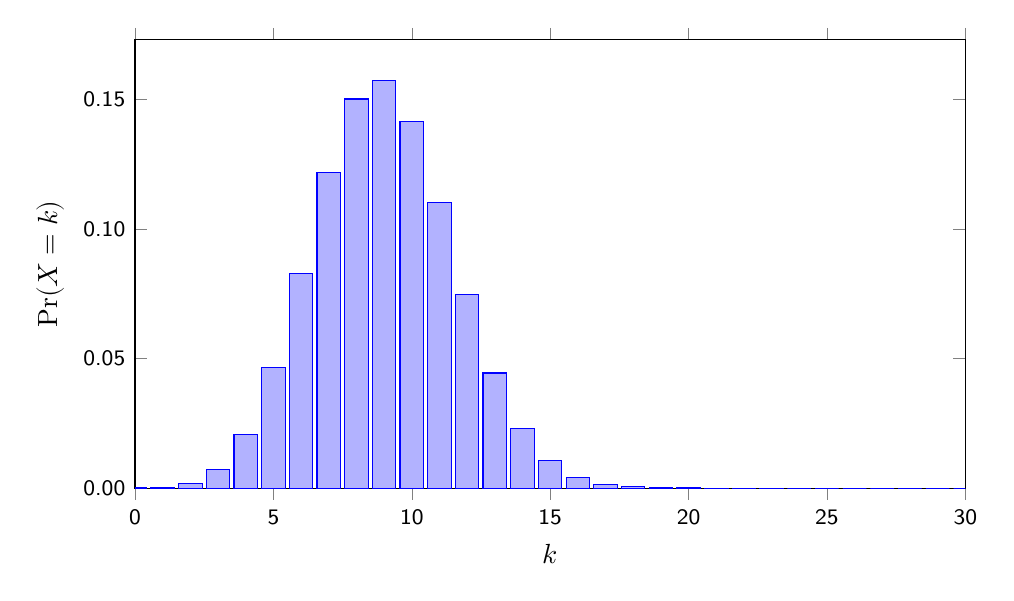
\begin{tikzpicture}[%
declare function={binom(\k,\n,\p)=\n!/(\k!*(\n-\k)!)*\p^\k*(1-\p)^(\n-\k);}]
\pgfmathsetmacro{\binomN}{30}
\begin{axis}[
    width=\textwidth, height=\axisdefaultheight,
    ylabel={$\Pr(X=k)$},
    xlabel={$k$},
    xmin=0, xmax=\binomN,
    ymin=0,
    scaled ticks = false,
    tick label style={/pgf/number format/assume math mode=true, font=\footnotesize\sffamily},
    yticklabel style={/pgf/number format/.cd, fixed, fixed zerofill, precision=2},
        domain=0:\binomN,samples at={0,1,...,\binomN},
    mark options={scale=0.75, blue},
    ybar, bar width = 8.5pt
        ]
%\addplot[ycomb] {binom(x,\binomN,0.3)};
\addplot {binom(x,\binomN,0.3)};
\end{axis}
\end{tikzpicture}
\end{frame}

\begin{frame}{二項分布}
\begin{align*}
\Pr(X = k) &= \binom{n}{k} p^k(1-p)^{n-k},\quad \emm{n=60},\, p=0.3.
\end{align*}
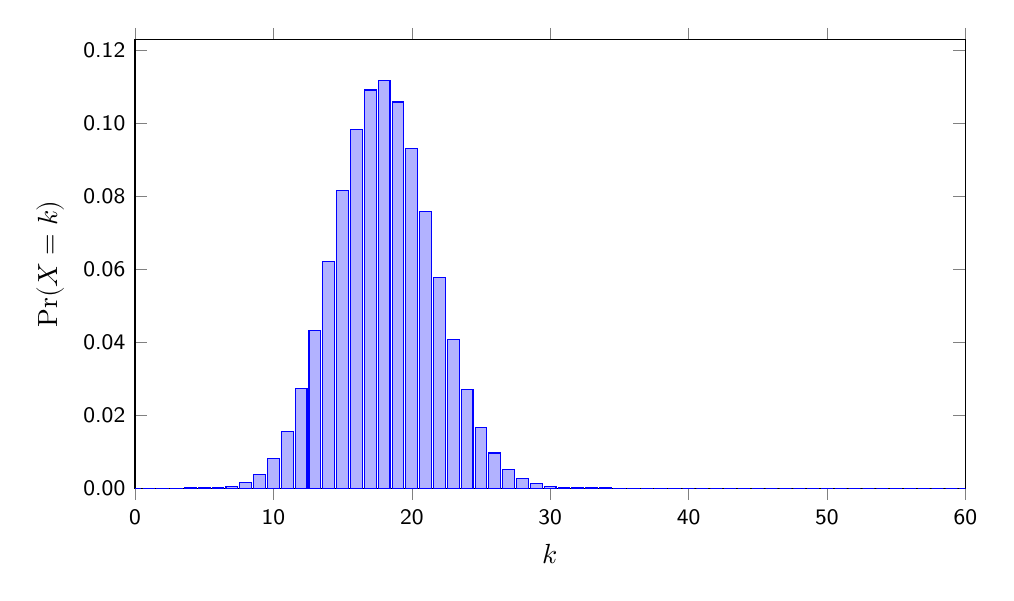
\begin{tikzpicture}[%
declare function={binom(\k,\n,\p)=\n!/(\k!*(\n-\k)!)*\p^\k*(1-\p)^(\n-\k);}]
\pgfmathsetmacro{\binomN}{60}
\begin{axis}[
    width=\textwidth, height=\axisdefaultheight,
    ylabel={$\Pr(X=k)$},
    xlabel={$k$},
    xmin=0, xmax=\binomN,
    ymin=0,
    scaled ticks = false,
    tick label style={/pgf/number format/assume math mode=true, font=\footnotesize\sffamily},
    yticklabel style={/pgf/number format/.cd, fixed, fixed zerofill, precision=2},
        domain=0:\binomN,samples at={0,1,...,\binomN},
    mark options={scale=0.75, blue},
    ybar, bar width = 4.25pt
        ]
%\addplot[ycomb] {binom(x,\binomN,0.3)};
\addplot {binom(x,\binomN,0.3)};
\end{axis}
\end{tikzpicture}
\end{frame}

\begin{frame}{二項分布}
\begin{align*}
\Pr(X = k) &= \binom{n}{k} p^k(1-p)^{n-k},\quad \emm{n=120},\, p=0.3.
\end{align*}
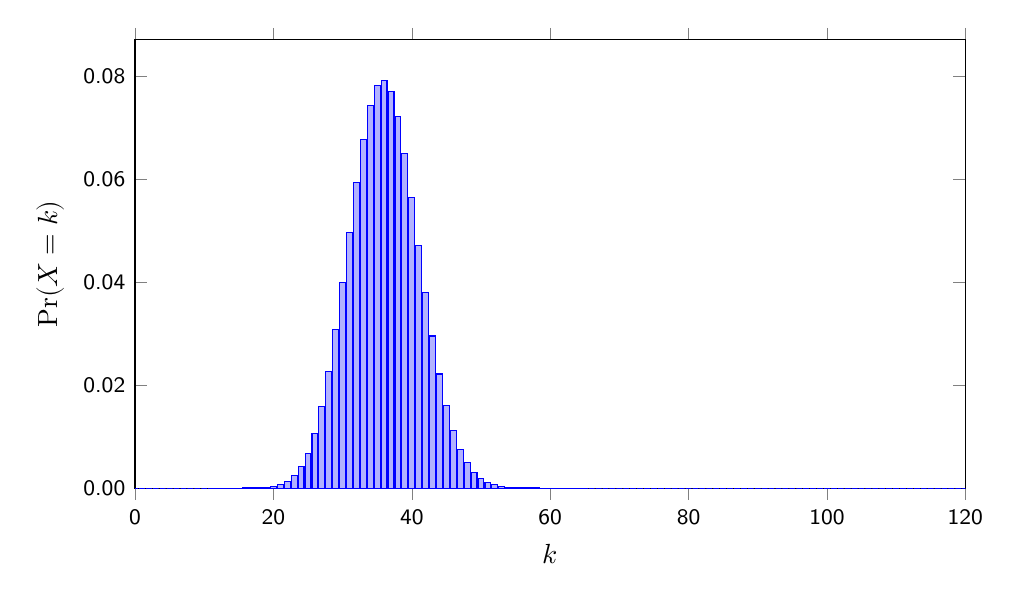
\begin{tikzpicture}[%
declare function={binom(\k,\n,\p)=\n!/(\k!*(\n-\k)!)*\p^\k*(1-\p)^(\n-\k);}]
\pgfmathsetmacro{\binomN}{120}
\begin{axis}[
    width=\textwidth, height=\axisdefaultheight,
    ylabel={$\Pr(X=k)$},
    xlabel={$k$},
    xmin=0, xmax=\binomN,
    ymin=0,
    scaled ticks = false,
    tick label style={/pgf/number format/assume math mode=true, font=\footnotesize\sffamily},
    yticklabel style={/pgf/number format/.cd, fixed, fixed zerofill, precision=2},
        domain=0:\binomN,samples at={0,1,...,\binomN},
    mark options={scale=0.75, blue},
    ybar, bar width = 2.125pt
        ]
%\addplot[ycomb] {binom(x,\binomN,0.3)};
\addplot {binom(x,\binomN,0.3)};
\end{axis}
\end{tikzpicture}
\end{frame}

\begin{frame}{二項分布}
\begin{align*}
\Pr(X = k) &= \binom{n}{k} p^k(1-p)^{n-k},\quad \emm{n=240},\, p=0.3.
\end{align*}
\begin{tikzpicture}[%
declare function={binom(\k,\n,\p)=\n!/(\k!*(\n-\k)!)*\p^\k*(1-\p)^(\n-\k);}]
\pgfmathsetmacro{\binomN}{240}
\pgfmathsetmacro{\p}{0.3}
\begin{axis}[
    width=\textwidth, height=\axisdefaultheight,
    ylabel={$\Pr(X=k)$},
    xlabel={$k$},
    xmin=0, xmax=\binomN,
    ymin=0,
    scaled ticks = false,
    tick label style={/pgf/number format/assume math mode=true, font=\footnotesize\sffamily},
    yticklabel style={/pgf/number format/.cd, fixed, fixed zerofill, precision=2},
        domain=0:\binomN,samples at={0,1,...,\binomN},
    mark options={scale=0.75, blue},
    ybar, bar width = .75pt
        ]
%\addplot[ycomb] {binom(x,\binomN,0.3)};
%\addplot {binom(x,\binomN,0.3)};
\addplot[domain=0:\binomN, color=blue, samples={\binomN+1}, thick] gnuplot { exp(lgamma(\binomN+1) - lgamma(x+1) - lgamma(\binomN-x+1) + x*log(\p) + (\binomN-x)*log(1-\p)) with impulses};
\end{axis}
\end{tikzpicture}
\end{frame}

\begin{frame}{二項分布}
\begin{align*}
\Pr(X = k) &= \binom{n}{k} p^k(1-p)^{n-k},\quad \emm{n=480},\, p=0.3.
\end{align*}
\begin{tikzpicture}[%
declare function={binom(\k,\n,\p)=\n!/(\k!*(\n-\k)!)*\p^\k*(1-\p)^(\n-\k);}]
\pgfmathsetmacro{\binomN}{480}
\pgfmathsetmacro{\p}{0.3}
\begin{axis}[
    width=\textwidth, height=\axisdefaultheight,
    ylabel={$\Pr(X=k)$},
    xlabel={$k$},
    xmin=0, xmax=\binomN,
    ymin=0,
    scaled ticks = false,
    tick label style={/pgf/number format/assume math mode=true, font=\footnotesize\sffamily},
    yticklabel style={/pgf/number format/.cd, fixed, fixed zerofill, precision=2},
        domain=0:\binomN,samples at={0,1,...,\binomN},
    mark options={scale=0.75, blue},
    ybar, bar width = .375pt
        ]
%\addplot[ycomb] {binom(x,\binomN,0.3)};
%\addplot {binom(x,\binomN,0.3)};
\addplot[domain=0:\binomN, color=blue, samples={\binomN+1}, thick] gnuplot { exp(lgamma(\binomN+1) - lgamma(x+1) - lgamma(\binomN-x+1) + x*log(\p) + (\binomN-x)*log(1-\p)) with impulses};
%\addplot[domain=0:\binomN, thick] gnuplot {x};
\end{axis}
\end{tikzpicture}
\end{frame}

\begin{frame}{二項分布}
\begin{align*}
\Pr(X = k) &= \binom{n}{k} p^k(1-p)^{n-k},\quad \emm{n=1000},\, p=0.3.
\end{align*}
\begin{tikzpicture}[%
declare function={binom(\k,\n,\p)=\n!/(\k!*(\n-\k)!)*\p^\k*(1-\p)^(\n-\k);}]
\pgfmathsetmacro{\binomN}{1000}
\pgfmathsetmacro{\p}{0.3}
\begin{axis}[
    width=\textwidth, height=\axisdefaultheight,
    ylabel={$\Pr(X=k)$},
    xlabel={$k$},
    xmin=0, xmax=\binomN,
    ymin=0,
    scaled ticks = false,
    tick label style={/pgf/number format/assume math mode=true, font=\footnotesize\sffamily},
    yticklabel style={/pgf/number format/.cd, fixed, fixed zerofill, precision=2},
        domain=0:\binomN,samples at={0,1,...,\binomN},
    mark options={scale=0.75, blue},
    ybar, bar width = .375pt
        ]
%\addplot[ycomb] {binom(x,\binomN,0.3)};
%\addplot {binom(x,\binomN,0.3)};
\addplot[domain=0:\binomN, color=blue, samples={\binomN+1}, thick] gnuplot { exp(lgamma(\binomN+1) - lgamma(x+1) - lgamma(\binomN-x+1) + x*log(\p) + (\binomN-x)*log(1-\p)) with impulses};
%\addplot[domain=0:\binomN, thick] gnuplot {x};
\end{axis}
\end{tikzpicture}
\end{frame}

\begin{frame}{二項分布}
\begin{align*}
\Pr(X = k) &= \binom{n}{k} p^k(1-p)^{n-k},\quad \emm{n=10000},\, p=0.3.
\end{align*}
\begin{tikzpicture}[%
declare function={binom(\k,\n,\p)=\n!/(\k!*(\n-\k)!)*\p^\k*(1-\p)^(\n-\k);}]
\pgfmathsetmacro{\binomN}{10000}
\pgfmathsetmacro{\p}{0.3}
\begin{axis}[
    width=\textwidth, height=\axisdefaultheight,
    ylabel={$\Pr(X=k)$},
    xlabel={$k$},
    xmin=0, xmax=\binomN,
    ymin=0,
    scaled ticks = false,
    tick label style={/pgf/number format/assume math mode=true, font=\footnotesize\sffamily},
    yticklabel style={/pgf/number format/.cd, fixed, fixed zerofill, precision=3},
        domain=0:\binomN,samples at={0,1,...,\binomN},
    mark options={scale=0.75, blue},
    ybar, bar width = .375pt
        ]
%\addplot[ycomb] {binom(x,\binomN,0.3)};
%\addplot {binom(x,\binomN,0.3)};
\addplot[domain=0:\binomN, color=blue, samples={\binomN+1}, thick] gnuplot { exp(lgamma(\binomN+1) - lgamma(x+1) - lgamma(\binomN-x+1) + x*log(\p) + (\binomN-x)*log(1-\p)) with impulses};
%\addplot[domain=0:\binomN, thick] gnuplot {x};
\end{axis}
\end{tikzpicture}
\end{frame}

\if0
\begin{frame}{二項分布}
\begin{align*}
\Pr(X = k) &= \binom{n}{k} p^k(1-p)^{n-k},\quad \emm{n=20000},\, p=0.3.
\end{align*}
\begin{tikzpicture}[%
declare function={binom(\k,\n,\p)=\n!/(\k!*(\n-\k)!)*\p^\k*(1-\p)^(\n-\k);}]
\pgfmathsetmacro{\binomN}{20000}
\pgfmathsetmacro{\p}{0.3}
\begin{axis}[
    width=\textwidth, height=\axisdefaultheight,
    ylabel={$\Pr(X=k)$},
    xlabel={$k$},
    xmin=0, xmax=\binomN,
    ymin=0,
    scaled ticks = false,
    tick label style={/pgf/number format/assume math mode=true, font=\footnotesize\sffamily},
    yticklabel style={/pgf/number format/.cd, fixed, fixed zerofill, precision=2},
        domain=0:\binomN,samples at={0,1,...,\binomN},
    mark options={scale=0.75, blue},
    ybar, bar width = .375pt
        ]
%\addplot[ycomb] {binom(x,\binomN,0.3)};
%\addplot {binom(x,\binomN,0.3)};
\addplot[domain=0:\binomN, color=blue, samples={\binomN+1}, thick] gnuplot { exp(lgamma(\binomN+1) - lgamma(x+1) - lgamma(\binomN-x+1) + x*log(\p) + (\binomN-x)*log(1-\p)) with impulses};
%\addplot[domain=0:\binomN, thick] gnuplot {x};
\end{axis}
\end{tikzpicture}
\end{frame}
\fi

\begin{frame}{二項分布}
\begin{align*}
\Pr(X = k) &= \binom{n}{k} p^k(1-p)^{n-k},\quad \emm{n=30},\, p=0.3.
\end{align*}
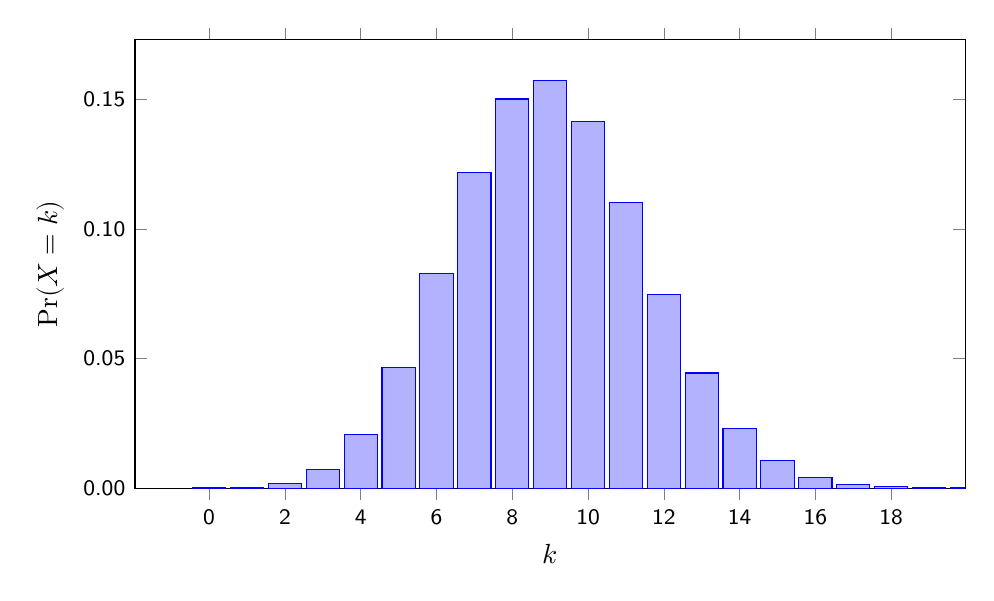
\begin{tikzpicture}[%
declare function={binom(\k,\n,\p)=\n!/(\k!*(\n-\k)!)*\p^\k*(1-\p)^(\n-\k);}]
\pgfmathsetmacro{\binomN}{30}
\pgfmathsetmacro{\p}{0.3}
\pgfmathsetmacro{\expect}{{\p*\binomN}}
\pgfmathsetmacro{\deviat}{{2*sqrt(\binomN)}}
\begin{axis}[
    width=\textwidth, height=\axisdefaultheight,
    ylabel={$\Pr(X=k)$},
    xlabel={$k$},
    xmin={\expect-\deviat}, xmax={\expect+\deviat},
    ymin=0,
    scaled ticks = false,
    tick label style={/pgf/number format/assume math mode=true, font=\footnotesize\sffamily},
    yticklabel style={/pgf/number format/.cd, fixed, fixed zerofill, precision=2},
        domain=0:\binomN,samples at={0,1,...,\binomN},
    mark options={scale=0.75, blue},
    ybar, bar width = 12pt
        ]
%\addplot[ycomb] {binom(x,\binomN,0.3)};
\addplot {binom(x,\binomN,\p)};
\end{axis}
\end{tikzpicture}
\end{frame}

\begin{frame}{二項分布}
\begin{align*}
\Pr(X = k) &= \binom{n}{k} p^k(1-p)^{n-k},\quad \emm{n=60},\, p=0.3.
\end{align*}
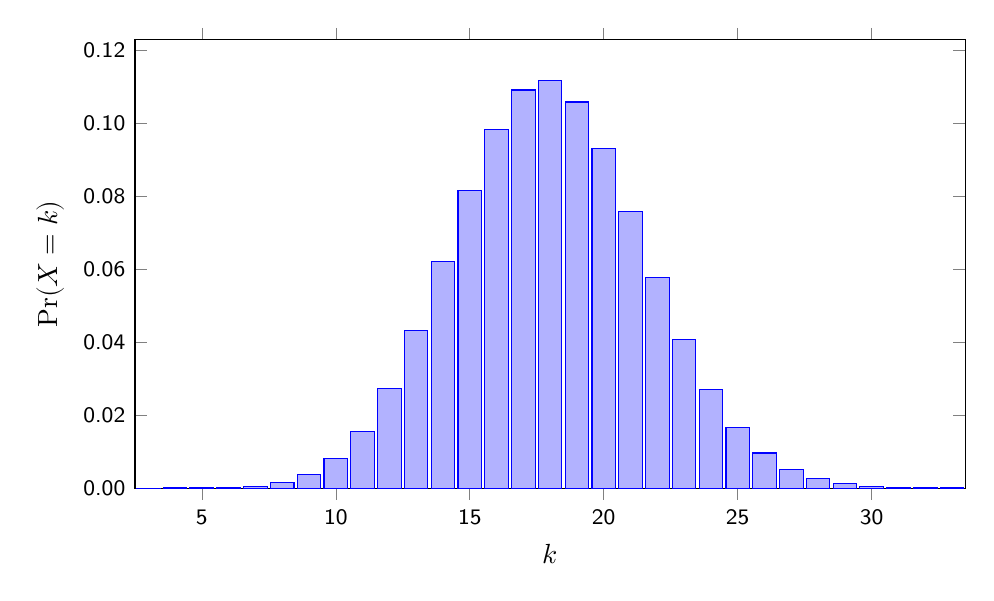
\begin{tikzpicture}[%
declare function={binom(\k,\n,\p)=\n!/(\k!*(\n-\k)!)*\p^\k*(1-\p)^(\n-\k);}]
\pgfmathsetmacro{\binomN}{60}
\pgfmathsetmacro{\p}{0.3}
\pgfmathsetmacro{\expect}{{\p*\binomN}}
\pgfmathsetmacro{\deviat}{{2*sqrt(\binomN)}}
\begin{axis}[
    width=\textwidth, height=\axisdefaultheight,
    ylabel={$\Pr(X=k)$},
    xlabel={$k$},
    xmin={\expect-\deviat}, xmax={\expect+\deviat},
    ymin=0,
    scaled ticks = false,
    tick label style={/pgf/number format/assume math mode=true, font=\footnotesize\sffamily},
    yticklabel style={/pgf/number format/.cd, fixed, fixed zerofill, precision=2},
        domain=0:\binomN,samples at={0,1,...,\binomN},
    mark options={scale=0.75, blue},
    ybar, bar width = 8.5pt
        ]
%\addplot[ycomb] {binom(x,\binomN,0.3)};
\addplot {binom(x,\binomN,\p)};
\end{axis}
\end{tikzpicture}
\end{frame}

\begin{frame}{二項分布}
\begin{align*}
\Pr(X = k) &= \binom{n}{k} p^k(1-p)^{n-k},\quad \emm{n=120},\, p=0.3.
\end{align*}
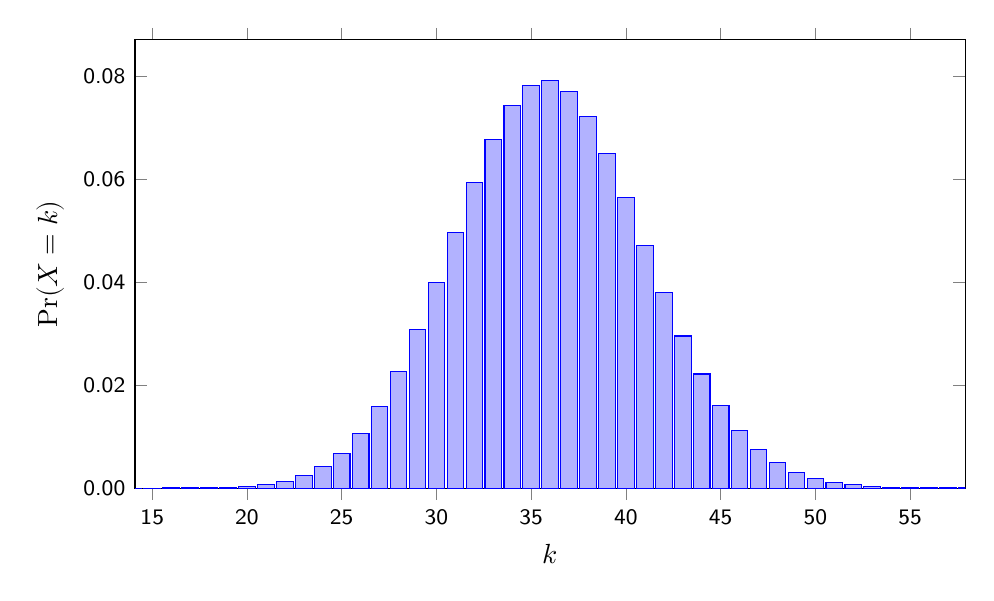
\begin{tikzpicture}[%
declare function={binom(\k,\n,\p)=\n!/(\k!*(\n-\k)!)*\p^\k*(1-\p)^(\n-\k);}]
\pgfmathsetmacro{\binomN}{120}
\pgfmathsetmacro{\p}{0.3}
\pgfmathsetmacro{\expect}{{\p*\binomN}}
\pgfmathsetmacro{\deviat}{{2*sqrt(\binomN)}}
\begin{axis}[
    width=\textwidth, height=\axisdefaultheight,
    ylabel={$\Pr(X=k)$},
    xlabel={$k$},
    xmin={\expect-\deviat}, xmax={\expect+\deviat},
    ymin=0,
    scaled ticks = false,
    tick label style={/pgf/number format/assume math mode=true, font=\footnotesize\sffamily},
    yticklabel style={/pgf/number format/.cd, fixed, fixed zerofill, precision=2},
        domain=0:\binomN,samples at={0,1,...,\binomN},
    mark options={scale=0.75, blue},
    ybar, bar width = 6pt
        ]
%\addplot[ycomb] {binom(x,\binomN,0.3)};
\addplot {binom(x,\binomN,\p)};
\end{axis}
\end{tikzpicture}
\end{frame}

\begin{frame}{二項分布}
\begin{align*}
\Pr(X = k) &= \binom{n}{k} p^k(1-p)^{n-k},\quad \emm{n=240},\, p=0.3.
\end{align*}
\begin{tikzpicture}[%
declare function={binom(\k,\n,\p)=\n!/(\k!*(\n-\k)!)*\p^\k*(1-\p)^(\n-\k);}]
\pgfmathsetmacro{\binomN}{240}
\pgfmathsetmacro{\p}{0.3}
\pgfmathsetmacro{\expect}{{\p*\binomN}}
\pgfmathsetmacro{\deviat}{{2*sqrt(\binomN)}}
\begin{axis}[
    width=\textwidth, height=\axisdefaultheight,
    ylabel={$\Pr(X=k)$},
    xlabel={$k$},
    xmin={\expect-\deviat}, xmax={\expect+\deviat},
    ymin=0,
    scaled ticks = false,
    tick label style={/pgf/number format/assume math mode=true, font=\footnotesize\sffamily},
    yticklabel style={/pgf/number format/.cd, fixed, fixed zerofill, precision=2},
        domain=0:\binomN,samples at={0,1,...,\binomN},
    mark options={scale=0.75, blue},
    ybar, bar width = 4.25pt
        ]
%\addplot[ycomb] {binom(x,\binomN,0.3)};
%\addplot {binom(x,\binomN,\p)};
\addplot[domain=0:\binomN, color=blue, samples={\binomN+1}, thick] gnuplot { exp(lgamma(\binomN+1) - lgamma(x+1) - lgamma(\binomN-x+1) + x*log(\p) + (\binomN-x)*log(1-\p)) with impulses};
\end{axis}
\end{tikzpicture}
\end{frame}

\begin{frame}{二項分布}
\begin{align*}
\Pr(X = k) &= \binom{n}{k} p^k(1-p)^{n-k},\quad \emm{n=480},\, p=0.3.
\end{align*}
\begin{tikzpicture}[%
declare function={binom(\k,\n,\p)=\n!/(\k!*(\n-\k)!)*\p^\k*(1-\p)^(\n-\k);}]
\pgfmathsetmacro{\binomN}{480}
\pgfmathsetmacro{\p}{0.3}
\pgfmathsetmacro{\expect}{{\p*\binomN}}
\pgfmathsetmacro{\deviat}{{2*sqrt(\binomN)}}
\begin{axis}[
    width=\textwidth, height=\axisdefaultheight,
    ylabel={$\Pr(X=k)$},
    xlabel={$k$},
    xmin={\expect-\deviat}, xmax={\expect+\deviat},
    ymin=0,
    scaled ticks = false,
    tick label style={/pgf/number format/assume math mode=true, font=\footnotesize\sffamily},
    yticklabel style={/pgf/number format/.cd, fixed, fixed zerofill, precision=2},
        domain=0:\binomN,samples at={0,1,...,\binomN},
    mark options={scale=0.75, blue},
    ybar, bar width = 3pt
        ]
%\addplot[ycomb] {binom(x,\binomN,0.3)};
%\addplot {binom(x,\binomN,\p)};
%\addplot[domain={\expect-\deviat}:{\expect+\deviat}, color=blue, samples={2*\deviat+1}, thick] gnuplot { exp(lgamma(\binomN+1) - lgamma(x+1) - lgamma(\binomN-x+1) + x*log(\p) + (\binomN-x)*log(1-\p)) with impulses};
\addplot[domain=0:\binomN, color=blue, samples={\binomN+1}, thick] gnuplot { exp(lgamma(\binomN+1) - lgamma(x+1) - lgamma(\binomN-x+1) + x*log(\p) + (\binomN-x)*log(1-\p)) with impulses};
\end{axis}
\end{tikzpicture}
\end{frame}

\begin{frame}{二項分布}
\begin{align*}
\Pr(X = k) &= \binom{n}{k} p^k(1-p)^{n-k},\quad \emm{n=1000},\, p=0.3.
\end{align*}
\begin{tikzpicture}[%
declare function={binom(\k,\n,\p)=\n!/(\k!*(\n-\k)!)*\p^\k*(1-\p)^(\n-\k);}]
\pgfmathsetmacro{\binomN}{1000}
\pgfmathsetmacro{\p}{0.3}
\pgfmathsetmacro{\expect}{{\p*\binomN}}
\pgfmathsetmacro{\deviat}{{2*sqrt(\binomN)}}
\begin{axis}[
    width=\textwidth, height=\axisdefaultheight,
    ylabel={$\Pr(X=k)$},
    xlabel={$k$},
    xmin={\expect-\deviat}, xmax={\expect+\deviat},
    ymin=0,
    scaled ticks = false,
    tick label style={/pgf/number format/assume math mode=true, font=\footnotesize\sffamily},
    yticklabel style={/pgf/number format/.cd, fixed, fixed zerofill, precision=2},
        domain=0:\binomN,samples at={0,1,...,\binomN},
    mark options={scale=0.75, blue},
    ybar, bar width = 2pt
        ]
%\addplot[ycomb] {binom(x,\binomN,0.3)};
%\addplot {binom(x,\binomN,\p)};
%\addplot[domain={\expect-\deviat}:{\expect+\deviat}, color=blue, samples={2*\deviat+1}, thick] gnuplot { exp(lgamma(\binomN+1) - lgamma(x+1) - lgamma(\binomN-x+1) + x*log(\p) + (\binomN-x)*log(1-\p)) with impulses};
\addplot[domain=0:\binomN, color=blue, samples={\binomN+1}, thick] gnuplot { exp(lgamma(\binomN+1) - lgamma(x+1) - lgamma(\binomN-x+1) + x*log(\p) + (\binomN-x)*log(1-\p)) with impulses};
\end{axis}
\end{tikzpicture}
\end{frame}

\begin{frame}{二項分布}
\begin{align*}
\Pr(X = k) &= \binom{n}{k} p^k(1-p)^{n-k},\quad \emm{n=10000},\, p=0.3.
\end{align*}
\begin{tikzpicture}[%
declare function={binom(\k,\n,\p)=\n!/(\k!*(\n-\k)!)*\p^\k*(1-\p)^(\n-\k);}]
\pgfmathsetmacro{\binomN}{10000}
\pgfmathsetmacro{\p}{0.3}
\pgfmathsetmacro{\expect}{{\p*\binomN}}
\pgfmathsetmacro{\deviat}{{2*sqrt(\binomN)}}
\begin{axis}[
    width=\textwidth, height=\axisdefaultheight,
    ylabel={$\Pr(X=k)$},
    xlabel={$k$},
    xmin={\expect-\deviat}, xmax={\expect+\deviat},
    ymin=0,
    scaled ticks = false,
    tick label style={/pgf/number format/assume math mode=true, font=\footnotesize\sffamily},
    yticklabel style={/pgf/number format/.cd, fixed, fixed zerofill, precision=3},
        domain=0:\binomN,samples at={0,1,...,\binomN},
    mark options={scale=0.75, blue},
    ybar, bar width = .4pt
        ]
%\addplot[ycomb] {binom(x,\binomN,0.3)};
%\addplot {binom(x,\binomN,\p)};
%\addplot[domain={\expect-\deviat}:{\expect+\deviat}, color=blue, samples={2*\deviat+1}, thick] gnuplot { exp(lgamma(\binomN+1) - lgamma(x+1) - lgamma(\binomN-x+1) + x*log(\p) + (\binomN-x)*log(1-\p)) with impulses};
\addplot[domain=0:\binomN, color=blue, samples={\binomN+1}, thick] gnuplot { exp(lgamma(\binomN+1) - lgamma(x+1) - lgamma(\binomN-x+1) + x*log(\p) + (\binomN-x)*log(1-\p)) with impulses};
\end{axis}
\end{tikzpicture}
\end{frame}

\if0
\begin{frame}{二項分布}
\begin{align*}
\Pr(X = k) &= \binom{n}{k} p^k(1-p)^{n-k},\quad \emm{n=10000},\, p=0.3.
\end{align*}
\begin{tikzpicture}[%
declare function={binom(\k,\n,\p)=\n!/(\k!*(\n-\k)!)*\p^\k*(1-\p)^(\n-\k);}]
\pgfmathsetmacro{\binomN}{10000}
\pgfmathsetmacro{\p}{0.3}
\pgfmathsetmacro{\expect}{{\p*\binomN}}
\pgfmathsetmacro{\deviat}{{sqrt(\binomN)}}
\begin{axis}[
    width=\textwidth, height=\axisdefaultheight,
    ylabel={$\Pr(X=k)$},
    xlabel={$k$},
    xmin={\expect-\deviat}, xmax={\expect+\deviat},
    ymin=0,
    scaled ticks = false,
    tick label style={/pgf/number format/assume math mode=true, font=\footnotesize\sffamily},
    yticklabel style={/pgf/number format/.cd, fixed, fixed zerofill, precision=3},
        domain=0:\binomN,samples at={0,1,...,\binomN},
    mark options={scale=0.75, blue},
    ybar, bar width = .4pt
        ]
%\addplot[ycomb] {binom(x,\binomN,0.3)};
%\addplot {binom(x,\binomN,\p)};
%\addplot[domain={\expect-\deviat}:{\expect+\deviat}, color=blue, samples={2*\deviat+1}, thick] gnuplot { exp(lgamma(\binomN+1) - lgamma(x+1) - lgamma(\binomN-x+1) + x*log(\p) + (\binomN-x)*log(1-\p)) with impulses};
\addplot[domain=0:\binomN, color=blue, samples={\binomN+1}, thick] gnuplot { exp(lgamma(\binomN+1) - lgamma(x+1) - lgamma(\binomN-x+1) + x*log(\p) + (\binomN-x)*log(1-\p)) with impulses};
%\addplot {exp(-(x-\expect)^2/(2*sqrt(\binomN)))};
\end{axis}
\end{tikzpicture}
\end{frame}
\fi

\begin{frame}{中心極限定理}
\small
\begin{theorem}[中心極限定理]
$X$が分散を持つと仮定する。
\begin{align*}
\lim_{N\to\infty}\Pr\left(\frac{\left(\sum_{k=1}^N X_k\right)-N\expt{X}}{\sqrt{\var{X}N}} \le x\right) &= \Phi(x)
=\frac1{\sqrt{2\pi}}\int_{-\infty}^x\mathrm{e}^{-\frac{t^2}2}\mathrm{d}t
\end{align*}
\end{theorem}
\begin{align*}
Y_k&:= \frac{X_k-\expt{X}}{\sqrt{\var{X}}}\qquad \text{for } k=1,2,\dotsc,N
\end{align*}
は期待値0、分散1に正規化した確率変数である。
中心極限定理の主張は
\begin{align*}
\lim_{N\to\infty}\Pr\left(\frac{\sum_{k=1}^N Y_k}{\sqrt{N}} \le x\right) &= \Phi(x)
\end{align*}
である。$N$で割るのではなくて$\sqrt{N}$で割ることで大数の法則よりも細かい部分を見ている。
\end{frame}

\begin{frame}{特性関数}
\begin{definition}[特性関数]
確率変数$X$の\emm{特性関数}$\varphi_X\colon\mathbb{R}\to\mathbb{C}$を以下で定義する。
\begin{align*}
\varphi_X(t) &:= \expt{\mathrm{e}^{itX}}.
\end{align*}
\end{definition}
モーメント母関数は存在するとは限らないが特性関数は(定義域を$\mathbb{R}$として)\emm{常に存在}する。

\vspace{2em}
$X$と$Y$の分布が同じ$\emm{\iff}\varphi_X=\varphi_Y$ (ルベーグ積分に基づいた議論が必要).

\vspace{2em}
$X$が$k$次モーメントを持つ$\iff$$\varphi_X$は0で$k$回微分できる。
\begin{align*}
\left.\frac{\mathrm{d}^k\varphi_X(t)}{\mathrm{d}t^k}\right|_{t=0} &= i^k \expt{X^k}.
\end{align*}

%\vspace{1em}
%第二特性関数
%\begin{align*}
%H_X(t) &:= \log\expt{\mathrm{e}^{itX}}
%\end{align*}
\end{frame}

\begin{frame}{$X$と$Y$の分布が同じ$\iff\varphi_X=\varphi_Y$ (台が有限の場合)}
確率変数の像が\emm{有限集合}のとき、
\begin{align*}
\varphi_X(t) &= \sum_{k\in \mathrm{Range}(X)} \Pr(X = k) \mathrm{e}^{itk}
\end{align*}
ここで、$\mathrm{Range}(X)$の最小値と最大値をそれぞれ$k_\mathsf{min}$と$k_\mathsf{max}$とおくと、
$k_\mathsf{max}-k_\mathsf{min}$次多項式$Q_X$を以下のように定義する。
\begin{align*}
Q_X(x) &= \sum_{k\in \mathrm{Range}(X)} \Pr(X = k) x^{k-k_{\mathsf{min}}}
\end{align*}
このとき、$Q_X(\mathrm{e}^{it}) = \varphi_X(t) \mathrm{e}^{-itk_\mathsf{min}}$である。
一般的に\emm{$n$次多項式は異なる$(n+1)$点での値から一意に定まる}(Vandermonde行列の正則性)。
よって特性関数から多項式$Q_X$が一意に定まり、$\Pr(X=k)$が一意に定まる。

\begin{center}
確率質量関数から特性関数への写像が\emm{単射}であることが分かった。
これは一般の確率変数について(確率密度関数が存在しない場合でも)成り立つ。
%(レヴィの連続性定理)
\end{center}
%\begin{align*}
%&\sum_{t} \varphi_X(t) \mathrm{e}^{-itu}\\
%=&\sum_{t} \sum_{k\in \mathrm{Im}(X)} \Pr(X = k) \mathrm{e}^{itk} \mathrm{e}^{-itu}\\
%=& \sum_{k\in \mathrm{Im}(X)} \Pr(X = k)\left(\sum_{t} \mathrm{e}^{it(k-u)}\right)
%\end{align*}
\end{frame}

\begin{frame}{コーシー分布の特性関数}
\end{frame}

\begin{frame}{分布の収束と特性関数の収束}
\begin{theorem}[レヴィの連続性定理]
確率変数の列$Z_1,Z_2,\dotsc$と確率変数$Z$について
\begin{align*}
\lim_{n\to\infty}\varphi_{Z_n}(t) = \varphi_Z(t)\qquad\forall t\in\mathbb{R}
\end{align*}
のとき、
\begin{align*}
\lim_{n\to\infty} \Pr(Z_n\le x) &= \Pr(Z\le x)\qquad\forall x\in\mathbb{R}
\end{align*}
\end{theorem}
\end{frame}

\begin{frame}{中心極限定理の証明}
\small
期待値0分散1のi.i.d.確率変数$Y_1,\dotsc,Y_N$と標準正規分布に従う確率変数$Z$について
\begin{align*}
\lim_{N\to\infty}\Pr\left(\frac{\sum_{k=1}^N Y_k}{\sqrt{N}} \le x\right) &= \Pr(Z\le x)
\end{align*}
を示すためには
\begin{align*}
\lim_{N\to\infty} \varphi_{\frac{\sum_kY_k}{\sqrt{N}}}(t) &= \varphi_Z(t) = -\frac{t^2}2
\end{align*}
を示せばよい。$Y$は分散を持つので$\varphi_Y$は0で二回微分できる。テイラーの定理($\varphi_Y$は$\mathbb{R}\to\mathbb{C}$の関数だけど)より
\begin{align*}
\varphi_{\frac{\sum_kY_k}{\sqrt{N}}}(t) &= 
\varphi_{\sum_kY_k}\left(\frac{t}{\sqrt{N}}\right)
= \varphi_Y\left(\frac{t}{\sqrt{N}}\right)^N\\
&= \left(\varphi_Y(0) + \varphi_Y'(0)\frac{t}{\sqrt{N}} + \frac{\varphi_Y''(0)}2\left(\frac{t}{\sqrt{N}}\right)^2 + o\left(\frac{1}{N}\right)\right)^N\\
&= \left(1 + \frac{1}2\frac{t^2}{N} + o\left(\frac{1}{N}\right)\right)^N
\stackrel{N\to\infty}{\longrightarrow} \mathrm{e}^{-\frac{t^2}2}
\end{align*}
\end{frame}

\begin{frame}{中心極限定理の意義}
たくさんの独立同分布の確率変数の和は\emm{期待値の近くでは正規分布のよう}に振る舞う。

\vspace{2em}
同分布という条件は緩められる。

\vspace{2em}
多くの不確かな要因からくる\emm{ノイズは正規分布}とみなすとよい近似になっている。
\end{frame}

\if0
\begin{frame}{集中不等式との比較}
\begin{align*}
%\Pr\left(\frac1N\sum_{k=1}^N X_k\ge \expt{X} + \frac{a}{\sqrt{N}}\right) &\le \mathrm{e}^{-\frac{\left(a/\sqrt{N}\right)^2}{2s^2}N}
\Pr\left(\frac1N\sum_{k=1}^N X_k\ge \expt{X} + \frac{a}{\sqrt{N}}\right) &\le \mathrm{e}^{-I_X\left(\expt{X}+\frac{a}{\sqrt{N}}\right)N}
\approx \mathrm{e}^{-\frac{I_X''(\expt{X})}2 a^2}
= \mathrm{e}^{-\frac{a^2}{2\var{X}}}\\
\Pr\left(\frac1N\sum_{k=1}^N X_k\ge \expt{X} + \frac{a}{\sqrt{N}}\right) &\to 
%1-\Phi\left(\frac{a}{\sqrt{\var{X}}}\right)
\frac1{\sqrt{2\pi}}\int_{\frac{a}{\sqrt{\var{X}}}}^\infty \mathrm{e}^{-\frac{x^2}2}\dx
\end{align*}
\begin{align*}
I_X\left(\expt{X}+\frac{a}{\sqrt{N}}\right)&=I_X(\expt{X}) + I_X'(\expt{X})\frac{a}{\sqrt{N}} + \frac{I_X''(\expt{X})}2\frac{a^2}N + o\left(\frac1N\right)\\
&= \frac1{2\var{X}}\frac{a^2}N + o\left(\frac1N\right)
\end{align*}
\end{frame}
\fi

\if0
\begin{frame}{中心極限定理の収束のスピード}
\begin{align*}
H_{\frac{\sum_kY_k}{\sqrt{N}}}(t) &= 
NH_Y\left(\frac{t}{\sqrt{N}}\right)\\
&=N\left(H_Y(0) + H_Y'(0)\frac{t}{\sqrt{N}} + \frac{H_Y''(0)}2\left(\frac{t}{\sqrt{N}}\right)^2 + o\left(\frac{1}{N}\right)\right)
= -\frac{t^2}2
\end{align*}
ここで$Y$が三次のキュムラントを持つとすると、テイラーの定理(ラグランジュ剰余項)よりある$\theta\in(0,t)$が存在して
\begin{align*}
H_{\frac{\sum_kY_k}{\sqrt{N}}}(t) &= 
N\left(H_Y(0) + H_Y'(0)\frac{t}{\sqrt{N}} + \frac{H_Y''(0)}2\left(\frac{t}{\sqrt{N}}\right)^2 + \frac{H_Y'''(\theta)}{3!} \left(\frac{t}{\sqrt{N}}\right)^3\right)\\
&=N\left(-\frac{t^2}2\frac1N - i\frac{\kappa_3(\theta)}{3!} \left(\frac{t}{\sqrt{N}}\right)^3\right)
=-\frac{t^2}2 - i\frac{\kappa_3(\theta)t^3}{3!\sqrt{N}}
\end{align*}
\end{frame}

\begin{frame}{特性関数と密度関数}

\begin{align*}
\varphi_{\frac{\sum_kY_k}{\sqrt{N}}}(t)
% &= \mathrm{e}^{-\frac{t^2}2 - i\frac{\kappa_3(\theta)t^3}{3!\sqrt{N}}}\\
 &= \mathrm{e}^{-\frac{t^2}2}\mathrm{e}^{-i\frac{\kappa_3(\theta)t^3}{3!\sqrt{N}}}\\
 &= \mathrm{e}^{-\frac{t^2}2}\left(1 {-i\frac{\kappa_3(\theta)t^3}{3!\sqrt{N}}}\right)\\
\end{align*}
\begin{align*}
q(x) &= \frac1{2\pi}\int_{-\infty}^\infty \mathrm{e}^{-ixt} \varphi_{\frac{\sum_kY_k}{\sqrt{N}}}(t)\mathrm{d}t\\
&= \frac1{2\pi}\int_{-\infty}^\infty \mathrm{e}^{-ixt} \mathrm{e}^{-\frac{t^2}2 - i\frac{\kappa_3(\theta)t^3}{3!\sqrt{N}}}\mathrm{d}t
\end{align*}
\end{frame}
\fi

\begin{frame}{正規分布の性質}
平均$\mu$、分散$\sigma^2$の正規分布の確率密度関数は
\begin{align*}
p(x) &= \frac1{\sqrt{2\pi\sigma^2}} \mathrm{e}^{-\frac{(x-\mu)^2}{2\sigma^2}}
\end{align*}
$X$が平均$\mu$、分散$\sigma^2$の正規分布に従うことを、\emm{$X\sim N(\mu,\sigma^2)$}と表す。

\begin{itemize}
\setlength{\itemsep}{2em}
\item 任意の$a\in\mathbb{R}$について$X\sim N(\mu,\sigma^2)$のとき$X+a\sim N(\mu+a,\sigma^2)$である。
\item 任意の$a\in\mathbb{R}$について$X\sim N(\mu,\sigma^2)$のとき$aX\sim N(a\mu,a^2\sigma^2)$である。
\item 独立な確率変数$X_1\sim N(\mu_1, \sigma_1^2)$と$X_2\sim N(\mu_2, \sigma_2^2)$について
$X_1+X_2\sim N(\mu_1+\mu_2, \sigma_1^2+\sigma_2^2)$である。
\end{itemize}
\end{frame}

\begin{frame}{$X+a$の確率密度関数}
\small
確率変数$X$が確率密度関数$p(x)$を持つとする。

このとき、$a\in\mathbb{R}$について確率変数$X+a$の確率密度関数は
\begin{align*}
\Pr(X+a \le x)&= \Pr(X\le x-a)\\
&=\int_{-\infty}^{x-a} p(t) \mathrm{d}t\\
&=\int_{-\infty}^{x} p(u-a) \mathrm{d}u\qquad(u = t+a)
\end{align*}
より$\emm{p(x-a)}$である。
\end{frame}

\begin{frame}{$aX$の確率密度関数}
\scriptsize

また、$a>0$について確率変数$aX$の確率密度関数は
\begin{align*}
\Pr(aX \le x)&= \Pr\left(X\le \frac{x}{a}\right)\\
&=\int_{-\infty}^{\frac{x}{a}} p(t) \mathrm{d}t\\
&=\int_{-\infty}^{x} p\left(\frac{u}{a}\right) \frac1a\mathrm{d}u\qquad(u = ta)
\end{align*}
より$\emm{\frac1a p\left(\frac{x}{a}\right)}$である。
%
また、$a<0$について確率変数$aX$の確率密度関数は
\begin{align*}
\Pr(aX \le x)&= \Pr\left(X\ge \frac{x}{a}\right)
=\int_{\frac{x}{a}}^\infty p(t) \mathrm{d}t\\
&=\int_{x}^{-\infty} p\left(\frac{u}{a}\right) \frac1a\mathrm{d}u\qquad(u = ta)\\
&=-\int_{-\infty}^x p\left(\frac{u}{a}\right) \frac1a\mathrm{d}u
\end{align*}
より$\emm{-\frac1a p\left(\frac{x}{a}\right)}$である。
よって一般の$a\in\mathbb{R}\setminus\{0\}$について$aX$の確率密度関数は$\emm{\frac1{|a|}p\left(\frac{x}{a}\right)}$である。
\end{frame}

\begin{frame}{$X+Y$の確率密度関数}
独立確率変数$X$と$Y$がそれぞれ確率密度関数$p_X$と$p_Y$を持つとする。
このとき、$X+Y$の確率密度関数は
\begin{align*}
\Pr(X+Y\le z) &= \int_{-\infty}^\infty p_Y(y) \Pr(X+y\le z) \mathrm{d}y\\
&= \int_{-\infty}^\infty  p_Y(y)  \left(\int_{-\infty}^{z-y}p_X(x) \mathrm{d}x\right)\mathrm{d}y\\
&= \int_{-\infty}^\infty  p_Y(y)  \left(\int_{-\infty}^{z}p_X(x'-y) \mathrm{d}x'\right)\mathrm{d}y\qquad(x'=x+y)\\
&= \int_{-\infty}^{z}\left(\int_{-\infty}^\infty  p_Y(y)  p_X(x'-y) \mathrm{d}y\right)\mathrm{d}x'\\
\end{align*}
より$\emm{\int_{-\infty}^{\infty} p_Y(y)p_X(x-y)\mathrm{d}y}$である。
これを確率密度関数$p_X$と$p_Y$の\emm{畳み込み}という。
\end{frame}

\begin{frame}{正規分布の密度関数}
\begin{align*}
p(x\emm{-a}) &= \frac1{\sqrt{2\pi\sigma^2}} \mathrm{e}^{-\frac{(x\emm{-a}-\mu)^2}{2\sigma^2}}\\
\frac1{|a|}p(\emm{a}x) &= \frac1{\sqrt{2\pi\emm{a^2}\sigma^2}} \mathrm{e}^{-\frac{(x/\emm{a}-\mu)^2}{2\sigma^2}}\\
&= \frac1{\sqrt{2\pi\emm{a^2}\sigma^2}} \mathrm{e}^{-\frac{(x-\emm{a}\mu)^2}{2\emm{a^2}\sigma^2}}\\
\int_{-\infty}^{\infty} p_{X_2}(y)p_{X_1}(x-y) \mathrm{d}y &=
\int_{-\infty}^{\infty} \frac1{\sqrt{2\pi\sigma_2^2}}\mathrm{e}^{-\frac{(y-\mu_2)^2}{2\sigma_2^2}} \frac1{\sqrt{2\pi\sigma_1^2}}\mathrm{e}^{-\frac{(x-y-\mu_1)^2}{2\sigma_1^2}} \mathrm{d}y\\
 &=
\int_{-\infty}^{\infty} \frac1{2\pi\sqrt{\sigma_1^2\sigma_2^2}}\mathrm{e}^{-\frac{\sigma_1^2(y-\mu_2)^2 - \sigma_2^2(x-y-\mu_1)^2}{2\sigma_1^2\sigma_2^2}}  \mathrm{d}y\\
\end{align*}
\end{frame}

\begin{frame}{特性関数を使った証明}
任意の独立確率変数$X$と$Y$と$a\in\mathbb{R}$について
\begin{align*}
\varphi_{X+a}(t) &= \expt{\mathrm{e}^{it(X+a)}} = \left(\expt{\mathrm{e}^{itX}}\cdot \mathrm{e}^{ita}\right) = \emm{\varphi_X(t) \mathrm{e}^{iat}}\\
\varphi_{aX}(t) &= \expt{\mathrm{e}^{it(aX)}} = \emm{\varphi_X(at)}\\
\varphi_{X+Y}(t) &= \expt{\mathrm{e}^{it(X+Y)}} =\expt{\mathrm{e}^{itX}}\expt{\mathrm{e}^{itY}} = \emm{\varphi_X(t) \varphi_Y(t)}
\end{align*}
$X\sim N(\mu,\sigma^2)$について
\begin{align*}
\varphi_X(t) &= \mathrm{e}^{i\mu t - \frac{\sigma^2t^2}2}
\end{align*}
より、
\begin{align*}
\varphi_{X\emm{+a}}(t) &= \mathrm{e}^{i(\mu\emm{+a}) t - \frac{\sigma^2t^2}2}\qquad\text{\small ($N(\mu+a,\sigma^2)$の特性関数)}\\
\varphi_{\emm{a}X}(t) &= \mathrm{e}^{i\mu \emm{a}t - \frac{\emm{a^2}\sigma^2t^2}2}\qquad\text{\small ($N(a\mu,a^2\sigma^2)$の特性関数)}\\
\varphi_{X_1\emm{+}X_2}(t) &= \mathrm{e}^{i(\mu_1\emm{+}\mu_2)t - \frac{(\sigma_1^2\emm{+}\sigma_2^2)t^2}2}\qquad\text{\small ($N(\mu_1+\mu_2,\sigma_1^2+\sigma_2^2)$の特性関数)}
\end{align*}
\end{frame}

\begin{frame}{ポアソン分布の再帰性}
確率変数$X$が平均$\lambda>0$のポアソン分布に従うことを$X\sim\mathrm{Poisson}(\lambda)$と表す。
\begin{lemma}
独立確率変数$X$と$Y$が$X\sim\mathrm{Poisson}(\lambda_1)$、$Y\sim\mathrm{Poisson}(\lambda_2)$のとき
$X+Y\sim\mathrm{Poisson}(\lambda_1+\lambda_2)$.
\end{lemma}
\begin{proof}
$Z\sim\mathrm{Poisson}(\lambda)$について$\varphi_Z(t)=\mathrm{e}^{\lambda(\mathrm{e}^{it}-1)}$より
\begin{align*}
\varphi_{X+Y}(t) &= \varphi_X(t)\varphi_Y(t)\\
&=\mathrm{e}^{\lambda_1(\mathrm{e}^{it}-1)}\mathrm{e}^{\lambda_2(\mathrm{e}^{it}-1)}\\
&=\mathrm{e}^{(\lambda_1+\lambda_2)(\mathrm{e}^{it}-1)}
\end{align*}
であり、これは$\mathrm{Poisson}(\lambda_1+\lambda_2)$に従う確率変数の特性関数であるため$X+Y\sim\mathrm{Poisson}(\lambda_1+\lambda_2)$.
\end{proof}
\end{frame}

\begin{frame}{ポアソン分布と中心極限定理}
$X\sim\mathrm{Poisson}(\lambda)$のとき、
$X_1+\dotsb+X_N\sim\mathrm{Poisson}(N\lambda)$である。
\begin{itemize}
\item $\varphi_X(t) = \mathrm{e}^{\lambda(\mathrm{e}^{it}-1)}$.
\item $\varphi_{X-\lambda}(t) = \mathrm{e}^{\lambda(\mathrm{e}^{it}-1-it)}$.
\item $\varphi_{\sum_{k=1}^N(X_k-\lambda)}(t) = \mathrm{e}^{\lambda(\mathrm{e}^{it}-1-it)N}$.
\item $\varphi_{\frac{\sum_{k=1}^N(X_k-\lambda)}{\sqrt{\lambda N}}}(t) = \mathrm{e}^{\lambda\left(\mathrm{e}^{i\frac{t}{\sqrt{\lambda N}}}-1-i\frac{t}{\sqrt{\lambda N}}\right)N}$.
\end{itemize}
\end{frame}

\if0
\begin{frame}{独立だけど同分布じゃない場合}
$X_k$が分散を持つと仮定する。
\begin{align*}
\lim_{N\to\infty}\Pr\left(\frac{\left(\sum_{k=1}^N (X_k-\expt{X_k}\right)}{\sqrt{\sum_{k=1}^N\var{X_k}}} \le x\right) &\stackrel{\large ?}{=} \Phi(x)
%=\frac1{\sqrt{2\pi}}\int_{-\infty}^x\mathrm{e}^{-\frac{t^2}2}\mathrm{d}t
\end{align*}
\end{frame}
\fi

\begin{frame}{複数の確率変数の確率密度関数}
\small
\begin{definition}
$p_{Z_1,\dotsc,Z_n}\colon \mathbb{R}\to\mathbb{R}$が
確率変数$Z_1,\dotsc,Z_n$の確率密度関数$\stackrel{\mathrm{def}}{\iff}$
\begin{align*}
\Pr(Z_1\le z_1, Z_2\le z_2,\dotsm Z_n\le z_n)&=
\int_{\substack{-\infty< x_1 \le z_1\\ -\infty< x_2\le z_2\\\vdots\\-\infty<x_n\le z_n}} p_{Z_1,\dotsc,Z_n}(x_1,x_2,\dotsc,x_n)\mathrm{d}{\symbf{x}_1^n}
\end{align*}
\end{definition}
%確率変数$Z_1,\dotsc,Z_n$が\emm{独立}のとき、
%\begin{align*}
%p_{Z_1,\dotsc,Z_n}(x_1,\dotsc,x_n)&=p_{Z_1}(x_1)p_{Z_2}(x_2)\dotsm p_{Z_n}(x_n)
%\end{align*}
%である。
一つの確率変数$Z_1$の確率密度関数は$\Pr(Z_1\le z_1) = \Pr(Z_1\le z_1, Z_2 <\infty,\dotsc, Z_n<\infty)$より
\begin{align*}
p_{Z_1}(x_1)&=
\int_{\substack{-\infty< x_s <\infty \;\forall s\ne 1}} p_{Z_1,\dotsc,Z_n}(x_1,x_2,\dotsc,x_n)\mathrm{d}{\symbf{x}_2^n}.
\end{align*}
他の$Z_k$の確率密度関数についても同様。
\end{frame}

\begin{frame}{独立確率変数}
\begin{align*}
\Pr(Z_1\le z_1, Z_2\le z_2,\dotsm Z_n\le z_n)&=
\Pr(Z_1\le z_1)\Pr(Z_2\le z_2)\dotsm \Pr(Z_n\le z_n)
\end{align*}
\begin{align*}
\int_{\substack{-\infty< x_1 \le z_1\\ -\infty< x_2\le z_2\\\vdots\\-\infty<x_n\le z_n}} p_{Z_1,\dotsc,Z_n}(x_1,x_2,\dotsc,x_n)\mathrm{d}{\symbf{x}_1^n}
&=
\end{align*}
\end{frame}

\begin{frame}{分散共分散行列}
\small
\begin{definition}[分散共分散行列]
確率変数$Z_1,\dotsc,Z_n$の\emm{分散共分散行列}(もしくは\emm{共分散行列})$\vc{\symbf{Z}}\in\mathbb{R}^{n\times n}$は
$(i,\,j)$成分に$\cov{Z_i,\,Z_j}=\expt{Z_iZ_j}-\expt{Z_i}\expt{Z_j}$を持つ行列である。
\end{definition}
\begin{align*}
\vc{\symbf{Z}}&=
\begin{bmatrix}
\var{Z_1}&\cov{Z_1,Z_2}&\cov{Z_1,Z_3}\\
\cov{Z_2,Z_1}&\var{Z_2}&\cov{Z_2,Z_3}\\
\cov{Z_3,Z_1}&\cov{Z_3,Z_2}&\var{Z_3}\\
\end{bmatrix}
\end{align*}
確率変数のベクトルや行列に対する$\expt{\cdot}$は成分毎に期待値を取ることを表す。
\begin{align*}
\symbf{Z} &= \begin{bmatrix}Z_1\\Z_2\\\vdots\\Z_n\end{bmatrix}&\text{とすると}\qquad
\expt{\symbf{Z}} &= \begin{bmatrix}\expt{Z_1}\\\expt{Z_2}\\\vdots\\\expt{Z_n}\end{bmatrix}
\end{align*}
である。
分散共分散行列は以下のように表せる。
\begin{align*}
\symbf{\Sigma}&=
\expt{\symbf{Z} \symbf{Z}^T} - \expt{\symbf{Z}}\expt{\symbf{Z}}^T
\end{align*}
\end{frame}

\begin{frame}{分散共分散行列の性質}
\begin{itemize}
\setlength{\itemsep}{2em}
\item $\vc{\symbf{Z}}$は対称行列である。
\item $\vc{\symbf{Z}}$は半正定値である。
\item $\vc{\symbf{Z}+\symbf{b}}=\vc{\symbf{Z}}$.
\item $\vc{A\symbf{Z}}=A\vc{\symbf{Z}}A^T$.
%\item $\vc{\symbf{Z}+\symbf{Y}}=\vc{\symbf{Z}} + \vc{\symbf{Y}} + $.
\end{itemize}
\end{frame}

\begin{frame}{線形変換の分散共分散行列}
行列$A\in\mathbb{R}^{m\times n}$と$n\times k$の確率変数行列$\symbf{Z}$について$\expt{A\symbf{Z}}=A\expt{\symbf{Z}}$である。
よって、$N$次元確率変数ベクトル$\symbf{Z}$について
\begin{align*}
&\expt{(\symbf{Z} - \expt{\symbf{Z}})(\symbf{Z} - \expt{\symbf{Z}})^T}\\
=&\expt{\symbf{Z}\symbf{Z}^T - \symbf{Z}\expt{\symbf{Z}}^T - \expt{\symbf{Z}}\symbf{Z}^T + \expt{\symbf{Z}}\expt{\symbf{Z}}^T}\\
=& \expt{\symbf{Z} \symbf{Z}^T} - \expt{\symbf{Z}}\expt{\symbf{Z}}^T
=\vc{\symbf{Z}}
\end{align*}
よって$\vc{\symbf{Z}+\symbf{b}}=\vc{\symbf{Z}}$である。

\vspace{1em}
\begin{align*}
\vc{A\symbf{Z}}&=\expt{\symbf{AZ} (\symbf{AZ})^T} - \expt{\symbf{AZ}}\expt{\symbf{AZ}}^T\\
&=A\expt{\symbf{Z} \symbf{Z}^T}A^T - A\expt{\symbf{Z}}\expt{\symbf{Z}}^TA^T\\
&=A\emm{\vc{\symbf{Z}}}A^T
\end{align*}
\end{frame}

\begin{frame}{分散共分散行列の半正定値性 I}
\small
\begin{align*}
&
\begin{bmatrix}
1&\expt{Z_1}&\expt{Z_2}&\expt{Z_3}\\
\expt{Z_1}&\expt{Z_1^2}&\expt{Z_1Z_2}&\expt{Z_1Z_3}\\
\expt{Z_2}&\expt{Z_2Z_1}&\expt{Z_2^2}&\expt{Z_2Z_3}\\
\expt{Z_3}&\expt{Z_3Z_1}&\expt{Z_3Z_2}&\expt{Z_3^2}\\
\end{bmatrix}\\
=&
\expt{
\begin{bmatrix}
1&Z_1&Z_2&Z_3\\
Z_1&Z_1^2&Z_1Z_2&Z_1Z_3\\
Z_2&Z_2Z_1&Z_2^2&Z_2Z_3\\
Z_3&Z_3Z_1&Z_3Z_2&Z_3^2\\
\end{bmatrix}}\\
=&
\expt{
\begin{bmatrix}
1\\
Z_1\\
Z_2\\
Z_3\\
\end{bmatrix}
\begin{bmatrix}
1&
Z_1&
Z_2&
Z_3
\end{bmatrix}}\ge 0\qquad (\text{半正定値行列の期待値は半正定値})
\end{align*}

任意の$\symbf{a}\in\mathbb{R}^n$ と$n\times n$半正定値ランダム行列$R$について
$\symbf{a}^T \expt{R}\symbf{a} = \expt{\symbf{a}^TR\symbf{a}}\ge 0$
なので$\expt{R}\ge0$.
\end{frame}

\begin{frame}{分散共分散行列の半正定値性 II}
\scriptsize
\begin{align*}
&
\begin{bmatrix}
-\expt{Z_1}&1&0&0\\
-\expt{Z_2}&0&1&0\\
-\expt{Z_3}&0&0&1\\
\end{bmatrix}
\begin{bmatrix}
1&\expt{Z_1}&\expt{Z_2}&\expt{Z_3}\\
\expt{Z_1}&\expt{Z_1^2}&\expt{Z_1Z_2}&\expt{Z_1Z_3}\\
\expt{Z_2}&\expt{Z_2Z_1}&\expt{Z_2^2}&\expt{Z_2Z_3}\\
\expt{Z_3}&\expt{Z_3Z_1}&\expt{Z_3Z_2}&\expt{Z_3^2}\\
\end{bmatrix}\\
=&
\begin{bmatrix}
0&\expt{Z_1^2}-\expt{Z_1}^2&\expt{Z_1Z_2}-\expt{Z_1}\expt{Z_2}&\expt{Z_1Z_3}-\expt{Z_1}\expt{Z_3}\\
0&\expt{Z_2Z_1}-\expt{Z_2}\expt{Z_1}&\expt{Z_2^2}-\expt{Z_2}^2&\expt{Z_2Z_3}-\expt{Z_2}\expt{Z_3}\\
0&\expt{Z_3Z_1}-\expt{Z_3}\expt{Z_1}&\expt{Z_3Z_2}-\expt{Z_3}\expt{Z_2}&\expt{Z_3^2}-\expt{Z_3}^2\\
\end{bmatrix}\\
\end{align*}
\begin{align*}
&
\begin{bmatrix}
0&\var{Z_1}&\cov{Z_1, Z_2}&\cov{Z_1, Z_3}\\
0&\cov{Z_2, Z_1}&\var{Z_2}&\cov{Z_2, Z_3}\\
0&\cov{Z_3, Z_1}&\cov{Z_3, Z_2}&\var{Z_3}
\end{bmatrix}
\begin{bmatrix}
-\expt{Z_1}& -\expt{Z_2}& -\expt{Z_3}\\
1&0&0\\
0&1&0\\
0&0&1\\
\end{bmatrix}\\
&=\vc{\symbf{Z}}
\end{align*}

$A\ge 0$のとき任意の行列$B$について$BAB^T\ge 0$なので$\vc{\symbf{Z}}\ge 0$である。
\end{frame}

\begin{frame}{多変量正規分布}
\begin{definition}[多変量正規分布]
確率変数$Z_1,\dotsc,Z_n$が平均$\symbf{\mu}\in\mathbb{R}^n$、分散共分散行列$\Sigma\in\mathbb{R}^{n\times n}$の多変量正規分布は確率密度関数
\begin{align*}
p_{\symbf{Z}}(\symbf{x}) &= \frac1{\sqrt{(2\pi)^n\det(\Sigma)}} \mathrm{e}^{-\frac12 (\symbf{x}-\symbf{\mu})^T\Sigma^{-1} (\symbf{x}-\symbf{\mu})}
\end{align*}
で定義される。
\end{definition}
\end{frame}

\begin{frame}{密度関数の積分}
\small
多変量正規分布の密度関数を積分して1になることを確認する。
$\Sigma$は対称行列なのである直交行列$V$と対角行列$D$が存在して$\Sigma=V^TDV$と表せる(スペクトル分解)。
また$\Sigma$は正定値なので、$D$の対角成分は正である。
\begin{align*}
&\int_{\mathbb{R}^n} \frac1{\sqrt{(2\pi)^n\det(\Sigma)}} \mathrm{e}^{-\frac12 (\symbf{x}-\symbf{\mu})^T\Sigma^{-1} (\symbf{x}-\symbf{\mu})}\mathrm{d}x\\
&=
\int_{\mathbb{R}^n} \frac1{\sqrt{(2\pi)^n\det(\Sigma)}} \mathrm{e}^{-\frac12 \symbf{x}^T\Sigma^{-1} \symbf{x}}\mathrm{d}x\\
&=
\int_{\mathbb{R}^n} \frac1{\sqrt{(2\pi)^n\det(D)}} \mathrm{e}^{-\frac12 (V\symbf{x})^TD^{-1} (V\symbf{x})}\mathrm{d}x\qquad(\Sigma=V^TDV)\\
&=
\int_{\mathbb{R}^n} \frac1{\sqrt{(2\pi)^n\det(D)}} \mathrm{e}^{-\frac12 \symbf{y}^TD^{-1} \symbf{y}}\frac1{|\det(V)|}\mathrm{d}y\qquad (y=Vx)\\
&=
\int_{\mathbb{R}^n} \frac1{\sqrt{(2\pi)^n\det(D)}} \mathrm{e}^{-\frac12 \symbf{z}^T \symbf{z}}\frac1{|\det(\sqrt{D^{-1}})|}\mathrm{d}z\qquad (z=\sqrt{D^{-1}}y)\\
&=
\int_{\mathbb{R}^n} \frac1{\sqrt{(2\pi)^n}} \mathrm{e}^{-\frac12 \symbf{z}^T \symbf{z}}\mathrm{d}z
=\prod_{k=1}^n\left(\int_{-\infty}^\infty \frac1{\sqrt{2\pi}}\mathrm{e}^{-\frac{z_k^2}2}\mathrm{d}z_k\right) = 1
\end{align*}
\end{frame}

\begin{frame}{多変数の特性関数}
\begin{definition}[多変数特性関数]
$n$次元確率変数$X$の\emm{特性関数}$\varphi_{X}\colon\mathbb{R}^n\to\mathbb{C}$を以下で定義する。
\begin{align*}
\varphi_{X}(t) &:= \expt{\mathrm{e}^{i\langle t,\, X\rangle}}.
\end{align*}
ここで$\langle t,\, X\rangle := \sum_{k=1}^n t_k X_k$である。
\end{definition}

\vspace{1em}
$X$と$Y$の分布が同じ$\emm{\iff}\varphi_X=\varphi_Y$ (ルベーグ積分に基づいた議論が必要).

\vspace{1em}
%$X$が$k$次モーメントを持つ$\iff$$\varphi_X$は0で$k$回微分できる。
\begin{align*}
%\left.\frac{\mathrm{d}^k\varphi_X(t)}{\mathrm{d}t^k}\right|_{t=0} &= i^k \expt{X^k}.
\left.\frac{\partial \varphi_X(t)}{\partial t_k}\right|_{t=0} &= \left.\expt{iX_k\mathrm{e}^{i\langle t,\, X\rangle}}\right|_{t=0} = i\expt{X_k}\\
\left.\frac{\partial^2 \varphi_X(t)}{\partial t_k\partial t_\ell}\right|_{t=0} &= \left.\expt{(iX_k)(iX_\ell)\mathrm{e}^{i\langle t,\, X\rangle}}\right|_{t=0} = -\expt{X_kX_\ell}.
\end{align*}
\end{frame}

\begin{frame}{多変数の特性関数の性質}
\begin{itemize}
\setlength{\itemsep}{1em}
\item $\varphi_{X+b}(t) = \varphi_X(t)\mathrm{e}^{i\langle t,\, b\rangle}\qquad\forall b\in\mathbb{R}^n$.
\item $\varphi_{AX}(t) = \varphi_X(A^Tt)\qquad\forall A\in\mathbb{R}^{m\times n}$.
\item $\varphi_{X+Y}(t) = \varphi_X(t)\varphi_Y(t)$.
\end{itemize}
\end{frame}

\begin{frame}{多変量正規分布の特性関数}
\small
\begin{align*}
&\expt{\mathrm{e}^{i\langle t,\,X\rangle}}\\
&=\int_{-\infty}^\infty \frac1{\sqrt{(2\pi)^n\det(\Sigma)}} \mathrm{e}^{-\frac12 (\symbf{x}-\symbf{\mu})^T\Sigma^{-1} (\symbf{x}-\symbf{\mu})}\mathrm{e}^{i\langle t,\, x\rangle}\mathrm{d}x\\
&= \int_{-\infty}^\infty \frac1{\sqrt{(2\pi)^n\det(\Sigma)}} \mathrm{e}^{-\frac12 \langle\Sigma^{-\frac12}(x-\mu),\,\Sigma^{-\frac12}(x-\mu)\rangle+i\langle \Sigma^{\frac12}t,\, \Sigma^{-\frac12}x\rangle}\mathrm{d}x\\
&= \int_{-\infty}^\infty \frac1{\sqrt{(2\pi)^n\det(\Sigma)}} \mathrm{e}^{-\frac12 \langle\Sigma^{-\frac12}(x-\mu-i\Sigma t),\,\Sigma^{-\frac12}(x-\mu-i\Sigma t)\rangle +i\langle \mu,\, t\rangle - \frac12\langle \Sigma^\frac12t,\,\Sigma^\frac12t\rangle}\mathrm{d}x\\
&= \mathrm{e}^{i\langle \mu,\, t\rangle - \frac12\langle \Sigma^\frac12t,\,\Sigma^\frac12t\rangle}
\end{align*}
\begin{align*}
\left.\frac{\partial \varphi_Z(t)}{\partial t_k}\right|_{t=0} &= i\mu_k\\
\left.\frac{\partial^2 \varphi_Z(t)}{\partial t_k\partial t_\ell}\right|_{t=0} &= 
\end{align*}
\end{frame}

\begin{frame}{多変量正規分布の一次変換}
\begin{lemma}
$n$次元の確率変数$\symbf{Z}\sim N(\symbf{\mu}, \Sigma)$のとき、
$A\symbf{Z}+\symbf{b}\sim N(A\symbf{\mu}+\symbf{b}, A\Sigma A^T)$.
%$Z_k\sim N(\mu_k, \Sigma_{k,k})$.
\end{lemma}
\begin{proof}
$\varphi_Z(t) = \mathrm{e}^{i\langle \mu,\, t\rangle - \frac12\langle \Sigma^\frac12t,\,\Sigma^\frac12t\rangle}$より、
\begin{align*}
\varphi_{AZ+b}(t) &= \varphi_{AZ}(t)\mathrm{e}^{i\langle t,\,b\rangle} = \varphi_Z(A^Tt)\mathrm{e}^{i\langle t,\,b\rangle}\\
&= \mathrm{e}^{i\langle \mu,\, A^T t\rangle - \frac12\langle \Sigma^\frac12A^T t,\,\Sigma^\frac12A^T t\rangle + i\langle t,\,b\rangle}\\
&= \mathrm{e}^{i\langle A\mu,\, t\rangle - \frac12\langle \Sigma^\frac12A^T t,\,\Sigma^\frac12A^T t\rangle+ i\langle t,\,b\rangle}\\
&= \mathrm{e}^{i\langle A\mu + b,\, t\rangle - \frac12\langle \Sigma^\frac12A^T t,\,\Sigma^\frac12A^T t\rangle}
\end{align*}
これは$N(A\mu+b,\, A\Sigma A^T)$の特性関数である。
\end{proof}
\end{frame}

\begin{frame}{多変量正規分布$\to$1変数正規分布}
\end{frame}

\end{document}
